\documentclass{beamer}
\usepackage{amsmath,amsbsy,amsopn,amstext,amsfonts,amssymb}
\usepackage{isomath}
\usepackage{ulem}
%\linespread{1.6}  % double spaces lines
\usepackage{graphicx}
\usepackage{subfigure}
\usepackage{color}
\usepackage{optidef}  % define optimization problems
\usepackage{multicol}  % multiple columns
\usepackage{listings} % for python code
\usepackage{mathrsfs}

\usepackage{polynom}
\newcommand{\adj}{\mathrm{adj}}
\newcommand{\constrainedmin}[3]{
		\begin{mini*}|s|
		{#2}{#1}{}{}
		\addConstraint{#3}
		\end{mini*}
}

\newcommand{\rwbcomment}[1]{{\color{blue}RWB:#1}}
\newcommand{\defeq}{\stackrel{\triangle}{=}}
\newcommand{\abs}[1]{\left|#1\right|}
\newcommand{\norm}[1]{\left\|#1\right\|}
\newcommand{\iprod}[1]{\left<#1\right>}
\newcommand{\ellbf}{\boldsymbol{\ell}}
\newcommand{\nubf}{\boldsymbol{\nu}}
\newcommand{\mubf}{\boldsymbol{\mu}}
\newcommand{\abf}{\mathbf{a}}
\newcommand{\bbf}{\mathbf{b}}
\newcommand{\cbf}{\mathbf{c}}
\newcommand{\dbf}{\mathbf{d}}
\newcommand{\ebf}{\mathbf{e}}
\newcommand{\fbf}{\mathbf{f}}
\newcommand{\gbf}{\mathbf{g}}
\newcommand{\hbf}{\mathbf{h}}
\newcommand{\ibf}{\mathbf{i}}
\newcommand{\jbf}{\mathbf{j}}
\newcommand{\kbf}{\mathbf{k}}
\newcommand{\lbf}{\mathbf{l}}
\newcommand{\mbf}{\mathbf{m}}
\newcommand{\nbf}{\mathbf{n}}
\newcommand{\obf}{\mathbf{o}}
\newcommand{\pbf}{\mathbf{p}}
\newcommand{\qbf}{\mathbf{q}}
\newcommand{\rbf}{\mathbf{r}}
\newcommand{\sbf}{\mathbf{s}}
\newcommand{\tbf}{\mathbf{t}}
\newcommand{\ubf}{\mathbf{u}}
\newcommand{\vbf}{\mathbf{v}}
\newcommand{\wbf}{\mathbf{w}}
\newcommand{\xbf}{\mathbf{x}}
\newcommand{\ybf}{\mathbf{y}}
\newcommand{\zbf}{\mathbf{z}}
\newcommand{\Jbf}{\mathbf{J}}
\newcommand{\Acal}{\mathcal{A}}
\newcommand{\Bcal}{\mathcal{B}}
\newcommand{\Lcal}{\mathcal{L}}
\newcommand{\Ncal}{\mathcal{N}}
\newcommand{\Rcal}{\mathcal{R}}
\definecolor{darkolivegreen}{rgb}{0.33, 0.42, 0.18}

\makeatletter
\newenvironment<>{proofstart}[1][\proofname]{%
    \par
    \def\insertproofname{#1\@addpunct{.}}%
    \usebeamertemplate{proof begin}#2}
  {\usebeamertemplate{proof end}}
\newenvironment<>{proofcont}{%
  \setbeamertemplate{proof begin}{\begin{block}{}}
    \par
    \usebeamertemplate{proof begin}}
  {\usebeamertemplate{proof end}}
\newenvironment<>{proofend}{%
    \par
    \pushQED{\qed}
    \setbeamertemplate{proof begin}{\begin{block}{}}
    \usebeamertemplate{proof begin}}
  {\popQED\usebeamertemplate{proof end}}
\makeatother

\title{ECEn 671: Mathematics of Signals and Systems}
\author{Randal W. Beard}
\institute{Brigham Young University}
\date{\today}

\begin{document}

%-------------------------------
\begin{frame}
	\titlepage
\end{frame}

%%%%%%%%%%%%%%%%%%%%%%%%%%%%%%%%%%%%%%%%%%%%%%%%%%%%%%%%%%%%%%%%%
\section{Singular Value Decomposition}
\frame{\sectionpage}


%----------------------------------
\begin{frame}\frametitle{Singular Value Decomposition}
	\begin{theorem}[Moon Theorem 7.1]
		Every matrix $A \in \mathbb{C}^{m\times n}$ can be factored as $A = U\Sigma V^H$ where $U \in \mathbb{C}^{m\times m}$ and $V \in \mathbb{C}^{n\times n}$ are unitary and $\Sigma \in \mathbb{R}^{m\times n}$ is diagonal with diagonal elements $\sigma_1 \geq \sigma_2 \geq cdots \geq \sigma_p \geq 0$.
	\end{theorem}
	
	\vfill
		
	The diagonal elements are called the singular values of $A$.  If $A$ is real then $U$ and $V$ are real and orthogonal.
\end{frame}

%----------------------------------
\begin{frame}\frametitle{Singular Value Decomposition, Proof}
	Note that the $A^HA$ is Hermitian, and positive definite because $x^HA^HAx = \norm{Ax }^2 \geq 0 \qquad \forall x\in\mathbb{C}^n$.
	
	\vfill
	
	So, from Chapter 6 we know that the eigenvalues of $A^HA$ are real with $m_i = q_i$ for each $\lambda_i$.  
	
	\vfill
	
	Let $(\lambda_i,\vbf_i)$ be an eigenpairs of $A^HA$ then
	\[ 
		A^HAV = V\Lambda \qquad \qquad V \text{-unitary} 
	\]
	where 
	\[
		V = \begin{pmatrix}
	    		\vbf_1 & \cdots & \vbf_n
			\end{pmatrix}, 
		\qquad \qquad
		\Lambda = \begin{pmatrix}
	    			\lambda_1 & & 0\\
	   		 		& \ddots &\\
	    			0 & & \lambda_n
	  			  \end{pmatrix}, 
	  \]
	  with
	  \[
	  	\lambda_1 \geq \lambda_2 \geq \cdots \geq \lambda_n.
	  \]
	
\end{frame}

%----------------------------------
\begin{frame}\frametitle{Singular Value Decomposition, Proof}
	Since the $rank(A^HA) \leq \min(m,n) = p$, then number of non-zero eigenvalues is $r \leq p$.
	
	For $1 \leq i \leq r$ let $\ubf_i = \frac{A\vbf_i}{\sqrt{\lambda_i}}$.
	
	Then 
	\begin{align*}
		\iprod{\ubf_i,\ubf_j } &= \iprod{\frac{A\vbf_i}{\sqrt{\lambda_i}}, \frac{A\vbf_j}{\sqrt{\lambda_j}} }
		= \frac{1}{\sqrt{\lambda_i\lambda_j}}\vbf_i^HA^HA\vbf_j\\
		&= \frac{\lambda_j}{\sqrt{\lambda_i\lambda_j}}\vbf_i^H\vbf_j 
		=  \delta_{ij}
	\end{align*}
	Use Gram-Schmidt to extend $\ubf_1,\ldots,\ubf_r$ to $[\ubf_1,\ldots,\ubf_m]$ such that $U = [\ubf_1, \ldots \ubf_m]$ is unitary.

\end{frame}

%----------------------------------
\begin{frame}\frametitle{Singular Value Decomposition, Proof}
%	\begin{columns}
%		\begin{column}{0.5\linewidth}
		\begin{lemma}
			If $(\lambda_i, \vbf_i)$ is an eigenpair of $A^H A$, then 
			$\ubf_i=\frac{A\vbf_i}{\sqrt{\lambda_i}}$ are eigenvectors of  $AA^H$.
		\end{lemma}
		\begin{center}
			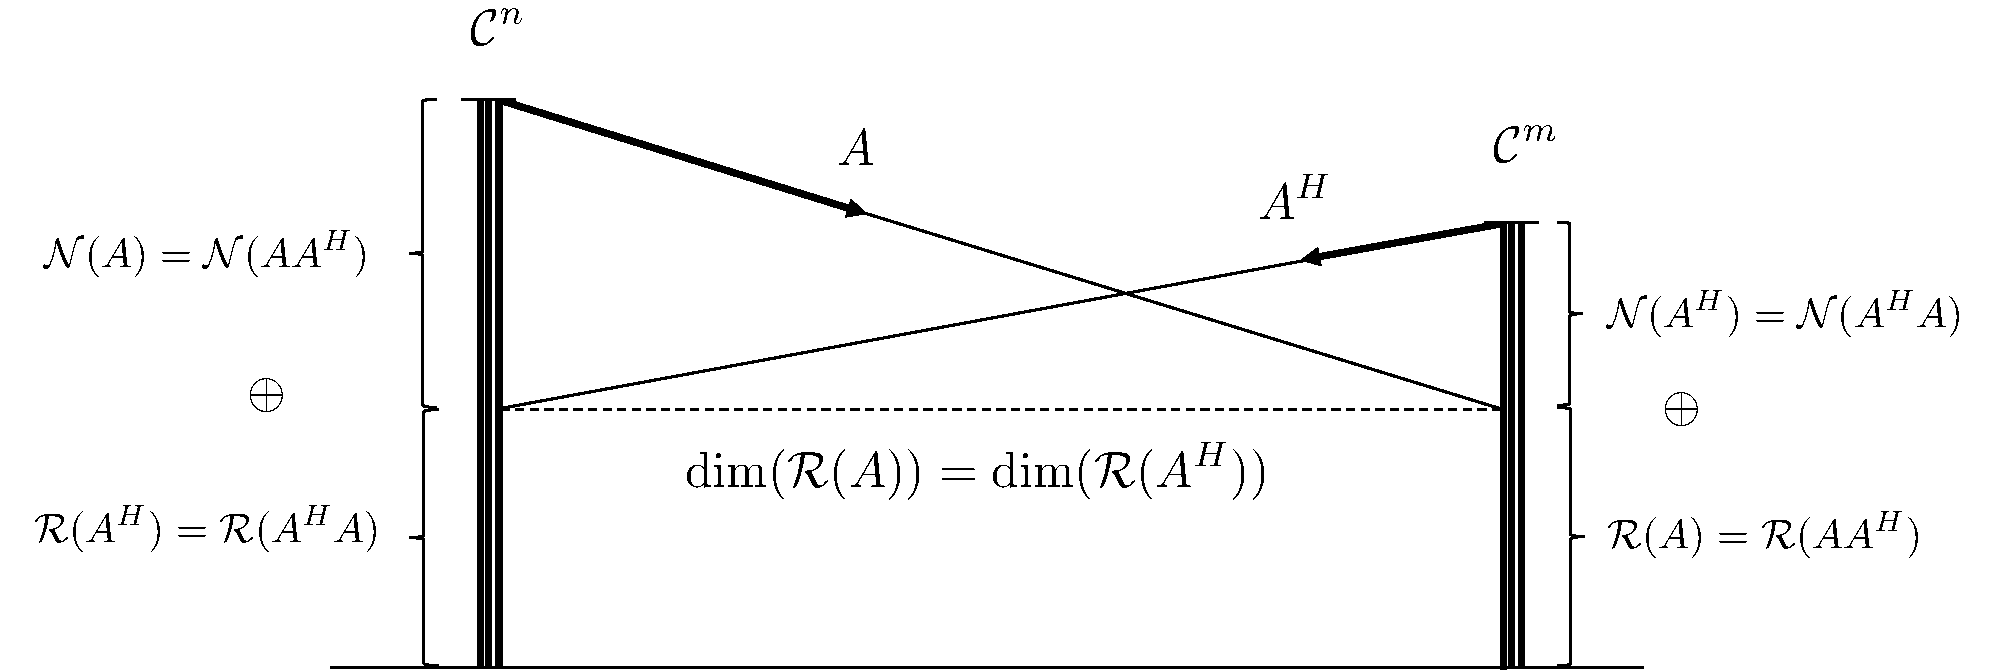
\includegraphics[width=0.5\textwidth]{figures/chap7_fundamental_subspace_1}
		\end{center}
%		\end{column}
%		\begin{column}{0.5\linewidth}
			\begin{proofstart}
				Note that since $\ubf_i = \frac{1}{\sqrt{\lambda_i}}A\vbf_i \qquad i = 1,\ldots,p$ then
				\begin{align*}
				& \ubf_i \in \mathcal{R}(A) \qquad i = 1, \ldots, p \\
				\implies & \ubf_i \in \mathcal{N}(A^H) \qquad i = p+1, \ldots, m \\
				\implies & \ubf_i \in \mathcal{N}(AA^H) \qquad i = p+1, \ldots, m \\
				\implies & AA^H\ubf_i = 0\cdot \ubf_i = 0 \\
				\implies & (0,\ubf_i) \text{~is an eigenpair of~} AA^H \qquad i = p+1,\ldots,m
				\end{align*}
			\end{proofstart}
%		\end{column}
%	\end{columns}
\end{frame}

%----------------------------------
\begin{frame}\frametitle{Singular Value Decomposition, Proof}
	Now lets look at
	\[ 
		U^HAV 
			= \begin{pmatrix}
	    		\ubf_1^H\\
	    		\vdots\\
	    		\ubf_m^H
	  		  \end{pmatrix}
	  		  A
	  		  \begin{pmatrix}
	    		\vbf_1 & \cdots & \vbf_n
	  		  \end{pmatrix} 
	  		= \begin{pmatrix}
	    		\ubf_1^HA\vbf_1 & \cdots & \ubf_1^HA\vbf_n\\
	    		\vdots & \ddots & \vdots\\
	    		\ubf_m^HA\vbf_1 & \cdots & \ubf_m^H\vbf_n
	  		  \end{pmatrix}.
	\]
	The $(i,j)^{th}$ element of $U^HAV$ is $\ubf_i^HA\vbf_j$.
	
	\vfill
	
	If $i \leq p$ then
	\begin{align*}
		\ubf_i^HA\vbf_j 
			&= \frac{1}{\sqrt{\lambda_i}}\vbf_i^HA^HA\vbf_j\\
			&= \frac{\lambda_j}{\sqrt{\lambda_i}}\vbf_i^H\vbf_j = \sqrt{\lambda_j}\delta_{ij}
	\end{align*}
\end{frame}

%----------------------------------
\begin{frame}\frametitle{Singular Value Decomposition, Proof}
	\begin{proofend}
		If $i > p$, then 
		\begin{align*}
			\ubf_i \in \mathcal{N}(A^H) &\Rightarrow A^H\ubf_i = 0 \\
			&\Rightarrow \ubf_i^HA = 0\\
			&\Rightarrow \ubf_i^H A \vbf_j = 0
		\end{align*}
		
		Therefore 
		\[
			U^HAV = \Sigma
		\]
		where $\Sigma = \text{diag}(\sigma_1, \ldots, \sigma_p)$ is real and diagonal, where $\sigma_j = 0$ when $j > p$.  Therefore
		\[
			A = U\Sigma V^H
		\] 
		as required.		
	\end{proofend}
\end{frame}

%----------------------------------
\begin{frame}\frametitle{Singular Value Decomposition}

	Note that the singular values of $A$ are the square root of the eigenvalues of $A^HA$ and $AA^H$.
	
	\vfill
	
	Also note that we can write 
	\[
	\Sigma 
		= \begin{pmatrix}
	    	\Sigma_1 & 0 \\
	    	0 & \Sigma_2
	  	  \end{pmatrix}
	  	= \begin{pmatrix}
 			\Sigma_1 & 0 \\
 			0 & 0	
 		  \end{pmatrix}
 	\]
	where
	\begin{align*}
		\Sigma_1 &= \underbrace{
						\text{diag}(\sigma_1, \dots, \sigma_p)
					}_{\mathbb{R}^{r\times r}} \\
		\Sigma_2 &= 0
	\end{align*}
\end{frame}

%----------------------------------
\begin{frame}\frametitle{Singular Value Decomposition}
	Then 
	\begin{align*}
	 A &= \begin{pmatrix}
	    	U_1 & U_2
	  	  \end{pmatrix}
	  	  \begin{pmatrix}
	    	\Sigma_1 & 0\\
	    	0 & 0
	      \end{pmatrix}
	      \begin{pmatrix}
	    	V_1^H\\
	    	V_2^H
	  	  \end{pmatrix}  \\
	&= \underbrace{U_1}_{m\times p}
	   \underbrace{\Sigma_1}_{p\times p}
	   \underbrace{V_1^H}_{n\times p} 
	   		\qquad \leftarrow\text{alternate form of SVD}\\
	&= \sum_{i=1}^p \sigma_i\ubf_i\vbf_i^H 
			\qquad \leftarrow\text{alternate form of SVD}
	\end{align*}	
	where $\ubf_i$'s are orthonormal and $\vbf_i$'s are orthonormal.
\end{frame}

%----------------------------------
\begin{frame}\frametitle{Singular Value Decomposition and Matrix Norm}
	Note that
	\begin{align*}
		\norm{A}_2 
			&= \sup_{\norm{x}_2=1}\norm{Ax}_2 
			= \sup_{\norm{x}_2=1}\sqrt{x^HA^HAx}\\
			&= \sup_{\norm{x}_2 = 1}\sqrt{x^HV_1\Sigma_1U_1^H U_1\Sigma_1V_1^Hx}\\
			&= \sup_{\norm{x}_2 = 1}\sqrt{x^HV_1\Sigma_1^2V_1^Hx}\\
			&= \sup_{\norm{x}_2 = 1}
				\sqrt{
					\begin{pmatrix}
		      			x^H\vbf_1 & \cdots & x^H\vbf_r
		    		\end{pmatrix}
		    		\begin{pmatrix}
		    			\sigma_1^2 & &\\
		    			& \ddots\\
		    			& & \sigma_p^2
		  			\end{pmatrix}
		  			\begin{pmatrix}
		    			\vbf_1^Hx\\
		    			\vdots\\
		    			\vbf_p^Hx
		  			\end{pmatrix}}  \\
		  	&= \sigma_1,
	\end{align*}	
	where the minimizer is $x = \vbf_1$.

\end{frame}

%----------------------------------
\begin{frame}\frametitle{Singular Value Decomposition and Rank}
	\begin{lemma}
		If $A \in \mathbb{C}^{m\times n}$, then 
		$\text{rank}(A) = p$ where $p$ is the number of non-zero singular values.
	\end{lemma}
	
	\begin{proof}
		\[ 
			\text{rank}(A) 
			= \text{rank}(U\Sigma V^H) 
			= \text{rank}(\Sigma) 
		\] 
		since $U$ and $V$ are both full rank.  
		Clearly $\text{rank}(\Sigma) = p$.
	\end{proof}
	
	
\end{frame}

%----------------------------------
\begin{frame}\frametitle{Singular Value Decomposition and Fundamental Subspaces}
	Fundamental subspace diagram:
	\begin{center}
		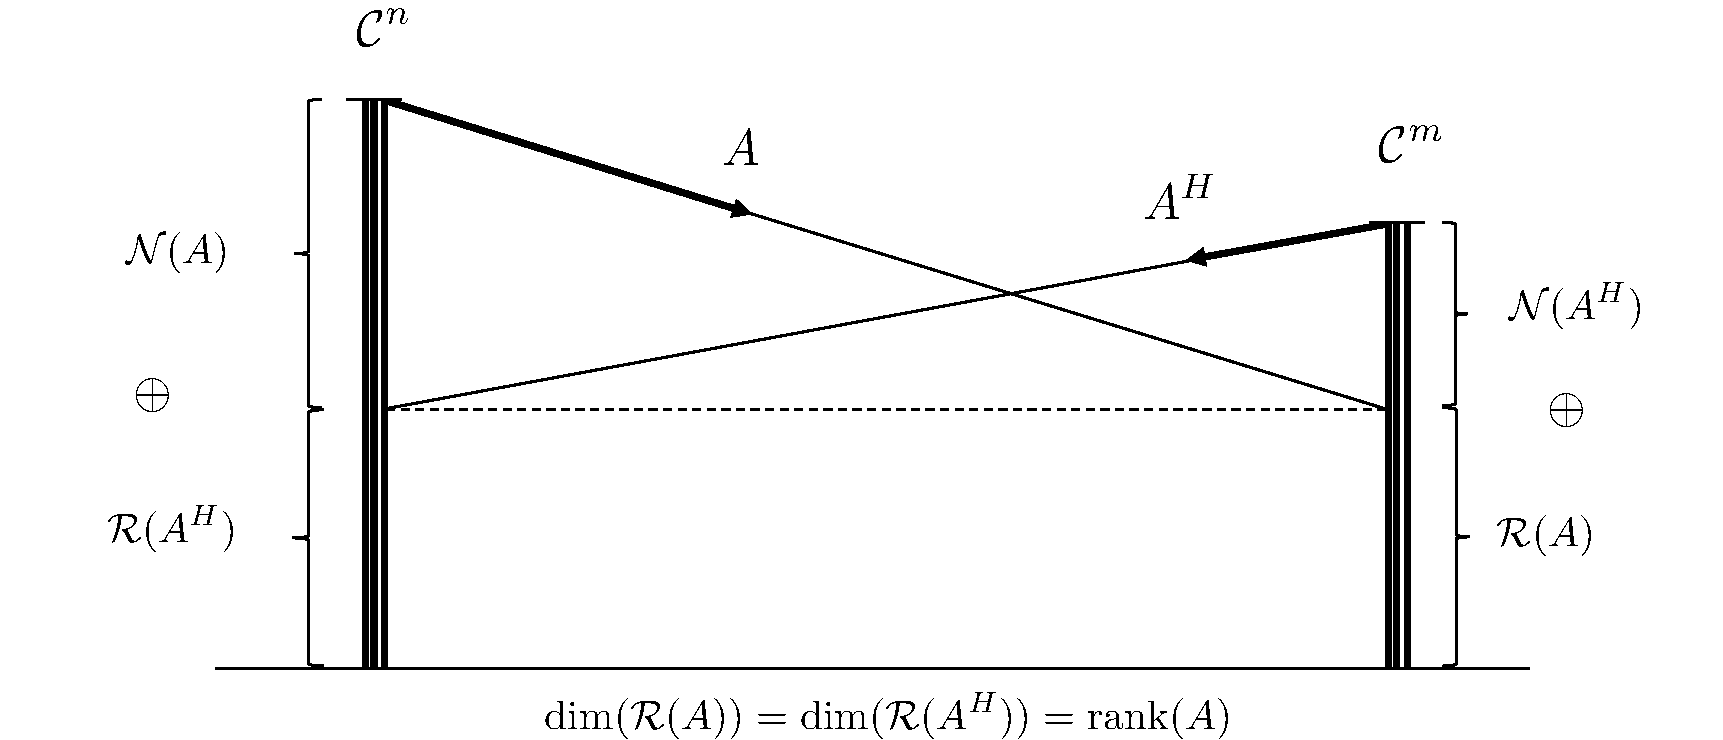
\includegraphics[width=0.9\textwidth]
			{figures/chap7_fundamental_subspace_2}
	\end{center}
	
	{\color{blue}Question:} 
		What information does the SVD provide?
		
	\vfill
	
	{\color{blue}Answer:} 
		The SVD completely characterizes all of the spaces.	
\end{frame}

%----------------------------------
\begin{frame}\frametitle{Singular Value Decomposition and Fundamental Subspaces}
	Given that 
	\[ 
		A = 
			\begin{pmatrix}
    			U_1 & U_2
  			\end{pmatrix}
  			\begin{pmatrix}
    			\Sigma_1 & 0\\
    			0 & 0
  			\end{pmatrix}
  			\begin{pmatrix}
    			V_1^H\\
    			V_2^H
  			\end{pmatrix}
  		= U_1\Sigma_1 V_1^H.
  	\]
	Let $y \in \mathcal{R}(A)$, then $\exists x \in \mathbb{C}^n$ such that $y = Ax$.  Which implies that 
	\begin{align*}
		y 
			&= U_1\Sigma_1V_1^Hx\\
			&= U_1z \text{ where } z = \Sigma_1V_1^Hx\\
			&= [\ubf_1 \cdots \ubf_p]
				\begin{pmatrix}
	    			z_1\\
	    			\vdots\\
	    			z_p
	  			\end{pmatrix} 
	  		= \ubf_1 z_1 + \cdots + \ubf_p z_p  \\
		\implies & y \in span\{\ubf_1, \cdots, \ubf_p\} \\
		\implies & \fbox{$\mathcal{R}(A) = span(U_1)$}
	\end{align*}
\end{frame}

%----------------------------------
\begin{frame}\frametitle{Singular Value Decomposition and Fundamental Subspaces}
	Since the columns of 
	$U_2$ 
	are orthonormal to 
	$U_1$ and 
	$\text{span}(U) = \mathbb{C}^m$ 
	and 
	$\mathcal{R}(A) \oplus \mathcal{N}(A^H) = \mathbb{C}^m$ 
	we must have that
	\[
		\fbox{$\mathcal{N}(A^H) = \text{span}(U_2)$}
	\]
	
	A similar argument shows that
	\[
		\fbox{$\mathcal{R}(A^H) = \text{span}(V_1)$}
	\]
	\[
		\fbox{$\mathcal{N}(A) = \text{span}(V_2)$}
	\]	
\end{frame}

%----------------------------------
\begin{frame}\frametitle{Singular Value Decomposition and Fundamental Subspaces}

	Therefore, the fundamental subspace diagram becomes
	\begin{center}
		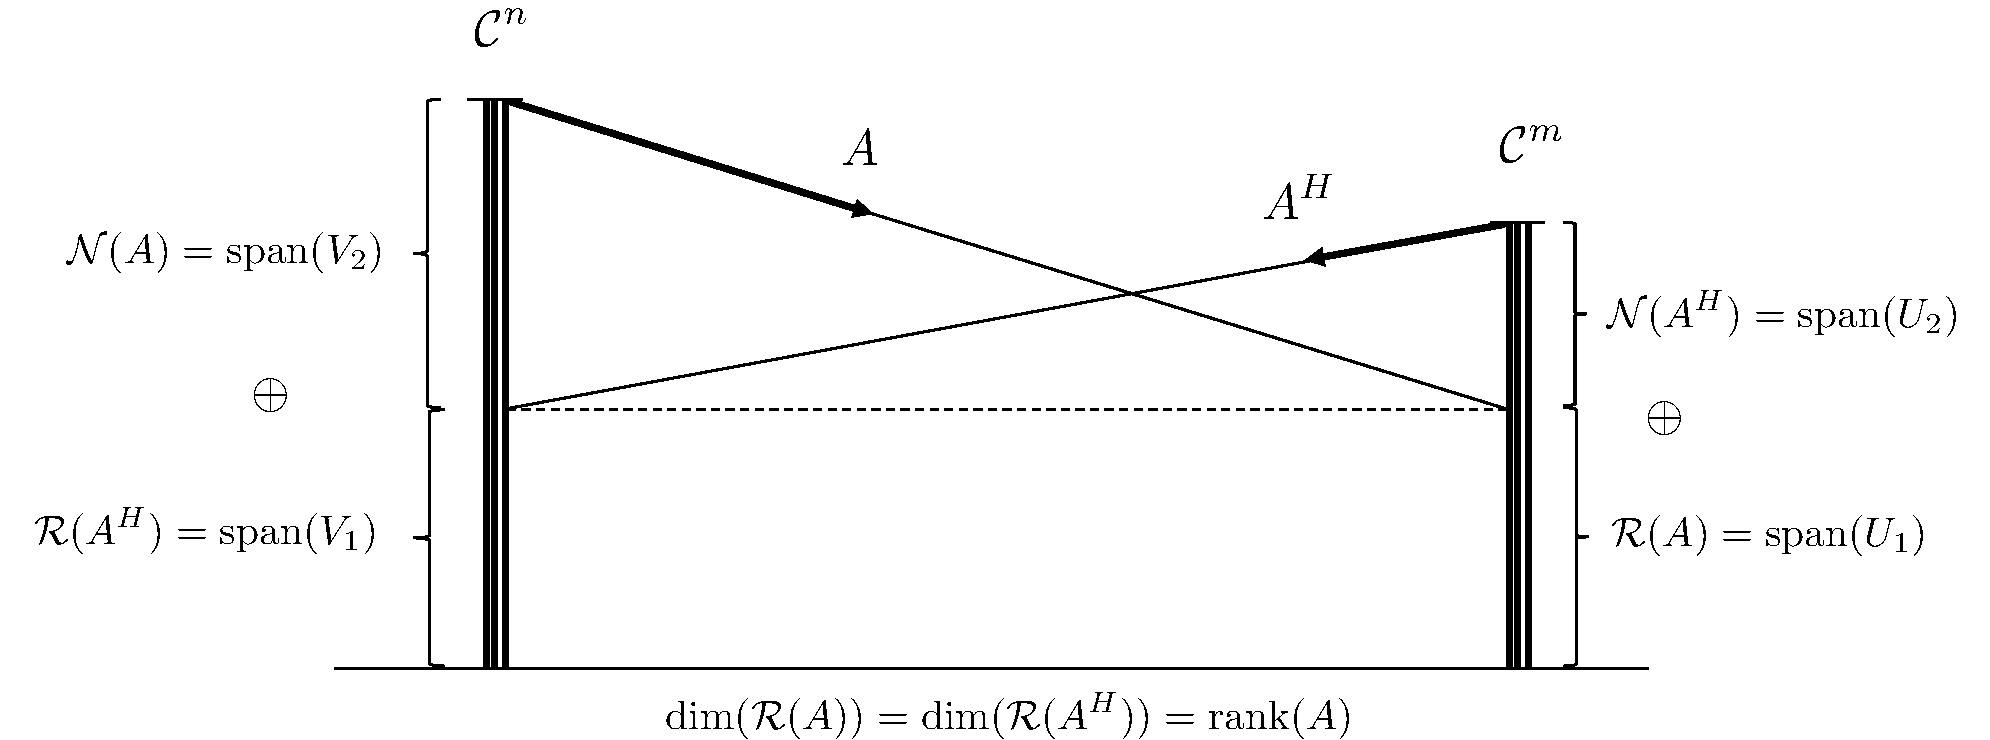
\includegraphics[width=0.99\textwidth]
			{figures/chap7_fundamental_subspace_3}	
	\end{center}
\end{frame}




\end{document}